The following sections describe the set of demos that have been compiled to
demonstrate some of the features and usage of the risk calculators of the
\glsdesc{acr:oqe}. These demos can be found in a public repository on GitHub at
the following link:
\href{https://github.com/gem/oq-engine/tree/master/demos/risk}
{https://github.com/gem/oq-engine/tree/master/demos/risk}.

These examples are purely demonstrative and are not intended to represent
accurately the seismicity, vulnerability or exposure characteristics of the
region selected, but simply to provide example input files that can be used
as a starting point for users planning to employ the \glsdesc{acr:oqe} in seismic
risk and loss estimation studies.

It is also noted that in the demonstrative examples presented in this section,
illustrations about the various messages from the engine displayed in the
command line interface are presented. These messages often contain information
about the calculation id and output id, which will certainly be different for
each user.

Following is the list of demos which illustrate how to use the \gls{acr:oqe} for
various scenario-based and probabilistic seismic damage and risk analyses:

\begin{itemize}

    \item ClassicalBCR
	\item ClassicalDamage
    \item ClassicalRisk
    \item EventBasedDamage
    \item EventBasedRisk
    \item ScenarioDamage
    \item ScenarioRisk

\end{itemize}

These seven demos use Nepal as the region of interest. An example
\gls{exposuremodel} has been developed for this region, comprising 9,063
assets distributed amongst 2,221 locations (due to the existence of more than
one \gls{asset} at the same location). A map with the distribution of the
number of buildings throughout Nepal is presented in Figure~\ref{fig:exposure-nepal}.

\begin{figure}[ht]
\centering
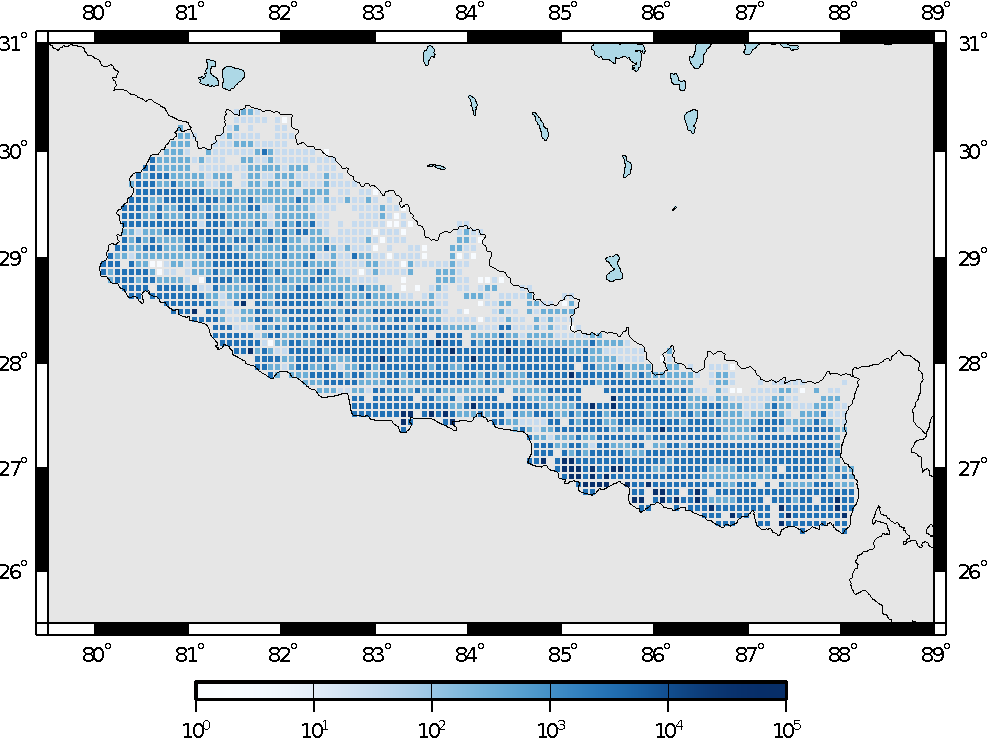
\includegraphics[width=12cm,height=8cm]{figures/risk/exposure-nepal.pdf}
\caption{Distribution of number of buildings in Nepal}
\label{fig:exposure-nepal}
\end{figure}

The building portfolio was organised into four classes for the rural areas
(adobe, dressed stone, unreinforced fired brick, wooden frames), and five
classes for the urban areas (the aforementioned typologies, in addition to
reinforced concrete buildings). For each one of these building typologies,
\glspl{vulnerabilityfunction} and \glspl{fragilityfunction} were collected
from the published literature available for the region. These input models are
only for demonstrative purposes and for further information about the building
characteristics of Nepal, users are advised to contact the National Society
for Earthquake Technology of Nepal (NSET -
\href{http://www.nset.org.np/}{http:www.nset.org.np/}).

The following sections include instructions not only on how to run the risk
calculations, but also on how to produce the necessary hazard inputs. Thus,
each demo comprises the configuration file, \gls{exposuremodel} and fragility or
vulnerability models fundamental for the risk calculations. Each demo folder
also a configuration file and the input models to produce the relevant hazard
inputs.


\section{Scenario Damage Demos}
\label{sec:demos_scenario_damage}
A rupture of magnitude Mw 7 in the central part of Nepal is considered in this
demo. The characteristics of this rupture (geometry, dip, rake, hypocentre,
upper and lower seismogenic depth) are defined in the \verb+fault_rupture.xml+
file, and the hazard and risk calculation settings are specified in the
\verb+job.ini+ file.

To run the Scenario Damage demo, users should navigate to the folder where the
required files have been placed and employ following command:

\begin{minted}[fontsize=\footnotesize,frame=single,bgcolor=lightgray]{shell-session}
user@ubuntu:~\$ oq engine --run job_hazard.ini,job_risk.ini
\end{minted}

The hazard calculation should produce the following outputs:

\begin{minted}[fontsize=\footnotesize,frame=single,bgcolor=lightgray]{shell-session}
Calculation 8967 completed in 4 seconds. Results:
  id | name
9060 | gmf_data
9061 | realizations
\end{minted}

and the following outputs should be produced by the risk calculation:

\begin{minted}[fontsize=\footnotesize,frame=single,bgcolor=lightgray]{shell-session}
Calculation 8968 completed in 16 seconds. Results:
  id | name
9062 | dmg_by_asset
9063 | losses_by_asset
\end{minted}


\section{Scenario Risk Demos}
\label{sec:demos_scenario_risk}
The same rupture described in the Scenario Damage demo is also used for this
demo. In this case, a combined job file, job.ini, is used to specify the
configuration parameters for the hazard and risk calculations.

To run the Scenario Risk demo, users should navigate to the folder where the
required files have been placed and employ following command:

\begin{minted}[fontsize=\footnotesize,frame=single,bgcolor=lightgray]{shell-session}
user@ubuntu:~\$ oq engine --run job.ini
\end{minted}

and the following outputs should be produced:

\begin{minted}[fontsize=\footnotesize,frame=single,bgcolor=lightgray]{shell-session}
Calculation 8970 completed in 16 seconds. Results:
  id | name
9070 | gmfs
9071 | realizations
9072 | loss_map-rlzs
9073 | agglosses-rlzs
\end{minted}


\section{Classical Probabilistic Seismic Damage Demos}
\label{sec:demos_classical_damage}
The seismic source model developed within the Global Seismic Hazard Assessment
Program (GSHAP) is used with the \cite{chiou2008} ground motion prediction
equation to produce the hazard input for this demo. No uncertainties are
considered in the seismic source model and since only one GMPE is being
considered, there will be only one possible path in the logic tree. Therefore,
only one set of seismic hazard curves will be produced. To run the hazard
calculation, the following command needs to be employed:

\begin{minted}[fontsize=\footnotesize,frame=single,bgcolor=lightgray]{shell-session}
user@ubuntu:~\$ oq engine --run job_hazard.ini
\end{minted}

which will produce the following sample hazard output:

\begin{minted}[fontsize=\footnotesize,frame=single,bgcolor=lightgray]{shell-session}
Calculation 8971 completed in 34 seconds. Results:
  id | name
9074 | hcurves
9075 | realizations
\end{minted}

The risk job calculates the probabilistic damage distribution for each asset
in the \gls{exposuremodel} starting from the above generated hazard curves. The
following command launches the risk calculations:

\begin{minted}[fontsize=\footnotesize,frame=single,bgcolor=lightgray]{shell-session}
user@ubuntu:~\$ oq engine --run job_risk.ini --hc 8971
\end{minted}

and the following sample outputs are obtained:

\begin{minted}[fontsize=\footnotesize,frame=single,bgcolor=lightgray]{shell-session}
Calculation 8972 completed in 16 seconds. Results:
  id | name
9076 | damages-rlzs
9077 | damages-stats
\end{minted}


\section{Classical Probabilistic Seismic Risk Demos}
\label{sec:demos_classical_risk}
The same hazard input as described in the Classical Probabilistic Damage demo
is used for this demo. Thus, the workflow to produce the set of hazard curves
described in Section~\ref{sec:demos_classical_damage} is also valid herein.
Then, to run the Classical Probabilistic Risk demo, users should navigate to
the folder containing the demo input models and configuration files and employ
the following command:

\begin{minted}[fontsize=\footnotesize,frame=single,bgcolor=lightgray]{shell-session}
user@ubuntu:~\$ oq engine --run job_hazard.ini
\end{minted}

which will produce the following hazard output:

\begin{minted}[fontsize=\footnotesize,frame=single,bgcolor=lightgray]{shell-session}
Calculation 8971 completed in 34 seconds. Results:
  id | name
9074 | hcurves
9075 | realizations
\end{minted}

In this demo, loss exceedance curves for each asset and two probabilistic loss
maps (for probabilities of exceedance of 1\% and 10\%) are produced. The
following command launches these risk calculations:

\begin{minted}[fontsize=\footnotesize,frame=single,bgcolor=lightgray]{shell-session}
user@ubuntu:~\$ oq engine --run job_risk.ini --hc 8971
\end{minted}

and the following outputs are expected:

\begin{minted}[fontsize=\footnotesize,frame=single,bgcolor=lightgray]{shell-session}
Calculation 8973 completed in 16 seconds. Results:
  id | name
9077 | loss_curves-stats
9078 | loss_maps-stats
9079 | avg_losses-stats
\end{minted}


\section{Event Based Probabilistic Seismic Damage Demos}
\label{sec:demos_event_based_damage}
This demo uses the same probabilistic seismic hazard assessment (PSHA) model
described in the previous examples in Section~\ref{sec:demos_classical_damage}
and Section~\ref{sec:demos_classical_risk}. However, instead of hazard curves,
sets of ground motion fields will be generated by the hazard calculation of
this demo. Again, since there is only one branch in the logic tree, only one
set of ground motion fields will be used in the risk calculations. The hazard
and risk jobs are defined in a single configuration file for this demo. To
trigger the hazard and risk calculations the following command needs to be
used:

\begin{minted}[fontsize=\footnotesize,frame=single,bgcolor=lightgray]{shell-session}
user@ubuntu:~\$ oq engine --run job.ini
\end{minted}

and the following results are expected:

\begin{minted}[fontsize=\footnotesize,frame=single,bgcolor=lightgray]{shell-session}
Calculation 2 completed in 29 seconds. Results:
  id | name
  24 | Aggregate Event Damages
  30 | Aggregate Event Losses
  20 | Average Asset Damages
  21 | Average Asset Damages Statistics
  22 | Average Asset Losses
  23 | Average Asset Losses Statistics
  32 | Earthquake Ruptures
  25 | Events
  26 | Full Report
  27 | Ground Motion Fields
  28 | Hazard Curves
  29 | Input Files
  31 | Realizations
\end{minted}


\section{Event Based Probabilistic Seismic Risk Demos}
\label{sec:demos_event_based_risk}
This demo uses the same probabilistic seismic hazard assessment (PSHA) model
described in the previous examples in Section~\ref{sec:demos_classical_damage}
and Section~\ref{sec:demos_classical_risk}. However, instead of hazard curves,
sets of ground motion fields will be generated by the hazard calculation of
this demo. Again, since there is only one branch in the logic tree, only one
set of ground motion fields will be used in the risk calculations. The hazard
and risk jobs are defined in a single configuration file for this demo. To
trigger the hazard and risk calculations the following command needs to be
used:

\begin{minted}[fontsize=\footnotesize,frame=single,bgcolor=lightgray]{shell-session}
user@ubuntu:~\$ oq engine --run job.ini
\end{minted}

and the following results are expected:

\begin{minted}[fontsize=\footnotesize,frame=single,bgcolor=lightgray]{shell-session}
Calculation 8974 completed in 229 seconds. Results:
  id | name
9079 | agg_curve-rlzs
9080 | agg_loss_table
9081 | loss_maps-rlzs
9082 | rcurves-rlzs
9083 | realizations
9084 | sescollection
\end{minted}


\section{Retrofit Benefit-Cost Ratio Demos}
\label{sec:demos_benefit_cost}
The loss exceedance curves used within this demo are produced using the
Classical Probabilistic Risk calculator. Thus, the process to produce the
seismic hazard curves described in Section~\ref{sec:demos_classical_risk} can
be employed here. Then, the risk calculations can be initiated using the
following command:

\begin{minted}[fontsize=\footnotesize,frame=single,bgcolor=lightgray]{shell-session}
user@ubuntu:~\$ oq engine --run job_risk.ini --hc 8971
\end{minted}

Alternatively, the hazard and risk jobs can be run sequentially using:

\begin{minted}[fontsize=\footnotesize,frame=single,bgcolor=lightgray]{shell-session}
user@ubuntu:~\$ oq engine --run job_hazard.ini,job_risk.ini
\end{minted}

which should produce the following output:

\begin{minted}[fontsize=\footnotesize,frame=single,bgcolor=lightgray]{shell-session}
Calculation 8976 completed in 14 seconds. Results:
  id | name
9087 | Benefit Cost Ratios
\end{minted}
